\chapter{Project Management}
\label{ch:projman}

\section{Project Plan}

% \begin{itemize}
%     \item link to gantt charts
%     \item explain buffer weeks
%     \item show actual gantt chart and explain differences
%     \item agile methodology, switchd to reuse after wseld
%     \item todo list to avoid forgetting stuff
% \end{itemize}

\subsection{Gantt Charts}

To plan a successful project, good time management is vital. A Gantt chart allows for a detailed view of how long each section is planned to take. This further enables accurate tracking of how well the project is progressing, such as whether it is behind or ahead of schedule.

The originally proposed Gantt chart for the project is shown below. Note that the Gantt chart shown in the start of Figure \ref{fig:original-gantt} was originally drafted before the full scope of the project was defined. It was assumed that this project would be developing a proof of concept DeepFake detection method and analysing its effectiveness rather than evaluating an existing detector.

\begin{figure}[h]
    \centering
    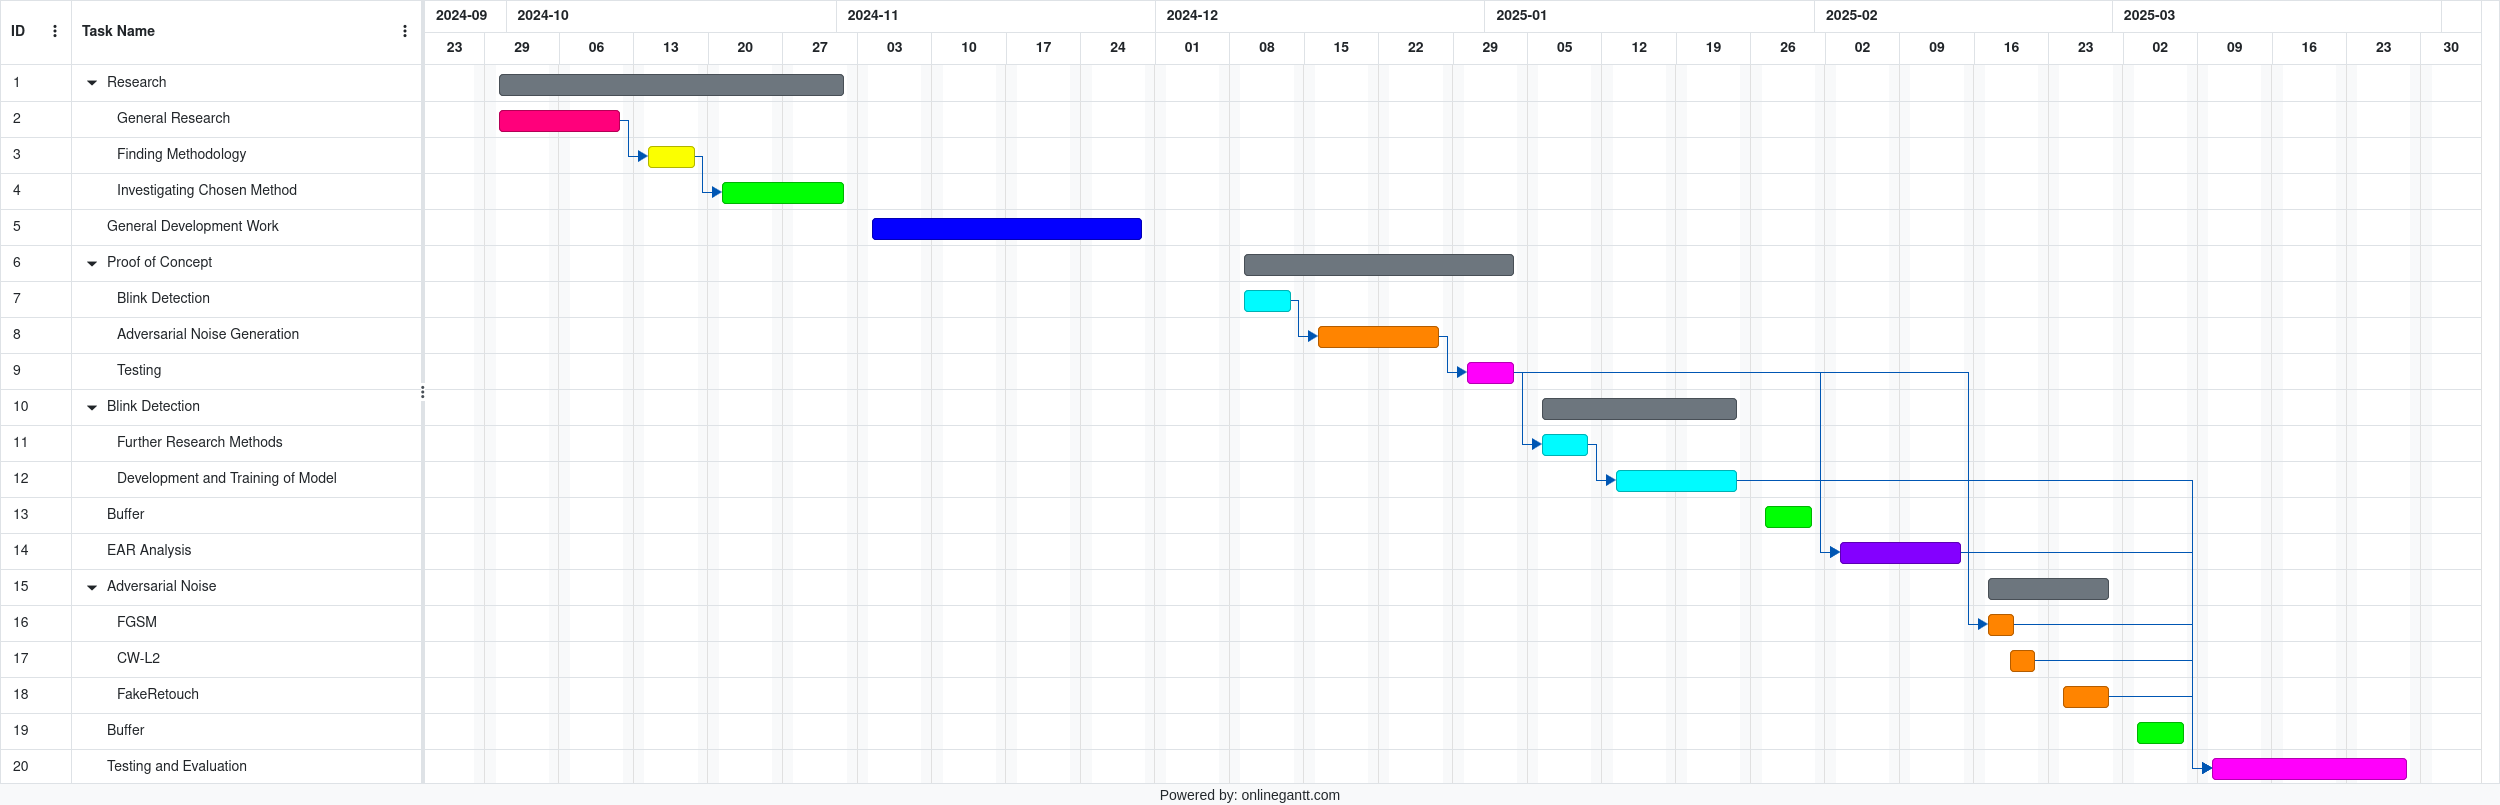
\includegraphics[width=1\linewidth]{dissertation/figures/original-gantt.png}
    \caption{The original Gantt chart planned for the software development section of the project}
    \label{fig:original-gantt}
\end{figure}

Most notable is the introduction of buffer weeks. The vast majority of projects will have unforeseeable events that will take longer to accomplish than originally planned: a piece of code might be particularly hard to implement, research in a particular area might be sparse resulting in source aggregation taking time. To account for these, buffer weeks are introduced at the end of major software development milestones to allow for potential delays.

The following Gantt chart is the actual timeline of the project.

\begin{figure}[h]
    \centering
    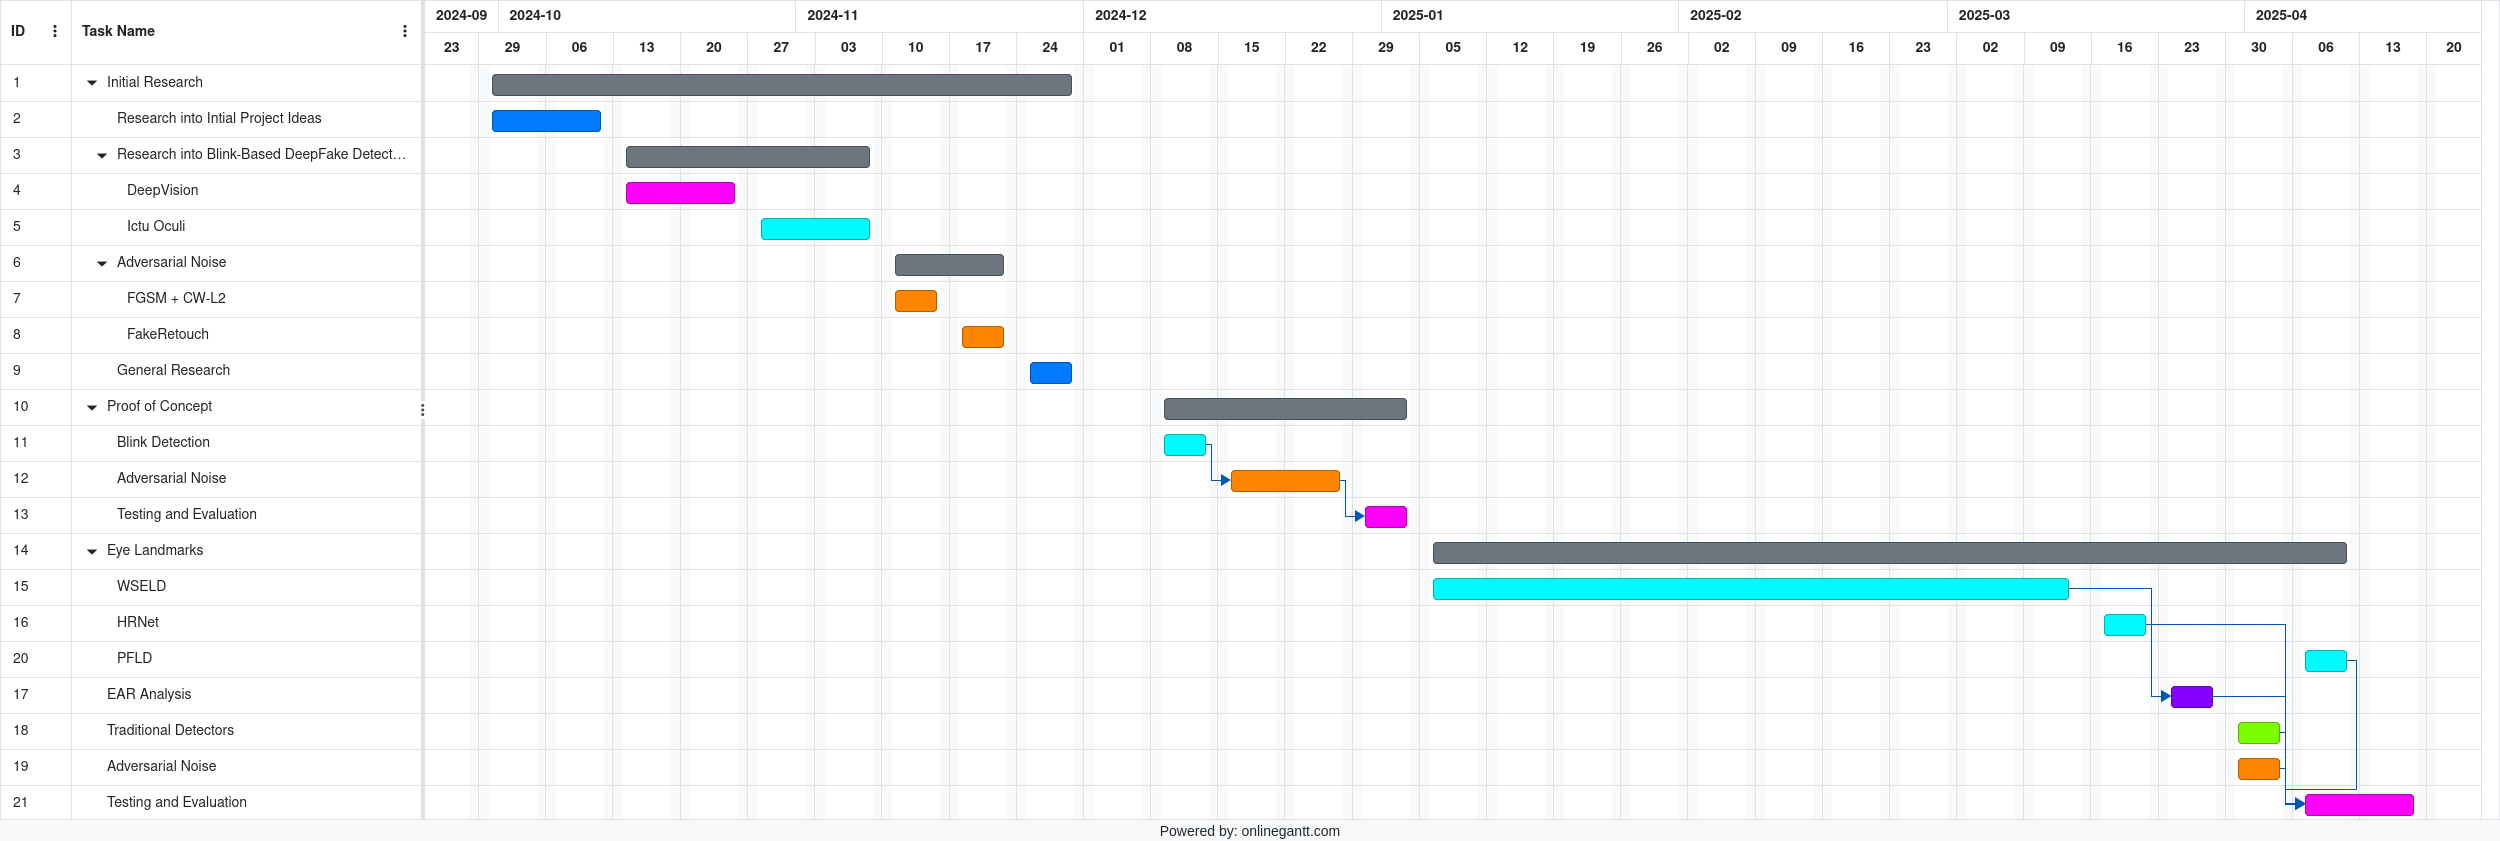
\includegraphics[width=1\linewidth]{dissertation/figures/actual-gantt.png}
    \caption{The actual Gantt chart for the software development section of the project}
    \label{fig:actual-gantt}
\end{figure}


\subsection{Dealing With Setbacks}

There are two main differences between the proposed Gantt chart and the actual one. Firstly is the length of time taken for research. This can be further decomposed into two more factors: workload from other courseworks and research required. 

It was originally believed that with effective time management and load balancing, that courseworks would not have any significant impact on the progress of the project. However some courseworks, most notable the coursework associated with CS325 Compiler Design, required more work than anticipated. As a result, work on the project was often delayed in order to free up time to focus on coursework. This led to the project being delayed by roughly two weeks. To remedy this, Wednesday afternoons were set aside as dedicated time to work on the project. Other times were also used if they were free. 

The initial project specification was written assuming that the project would only implement an existing DeepFake detection methodology that only existed as a theoretical proof of concept. The chosen methodology, blink detection, involves two models: one to determine the state of the eyes, and the other to determine whether the sequence produced by the previous model is feasible. Additionally, methods to add adversarial noise to images needed to be researched. Thus, the research phase took three weeks rather than the intended two, further setting the project behind.

The other major setback was the failed implementation of WSELD. Due to the various difficulties in implementing WSELD discussed in Section \ref{sec:sweld}, it was decided to switch to a different landmarking model. At that time approximately one month of work had gone into the failed development of the model. Whilst some of this work, such as normalising eye landmarking datasets and experience with TensorFlow, was transferable, the majority of work was not. Thus, the project was delayed by approximately three weeks. 

This was primarily mitigated using the buffer weeks built into the Gantt chart. Hence, the overall delay was reduced from three weeks to one, which was much more manageable. To speed up design of its replacements, it was decided to switch to a reuse-oriented methodology. As such, models were only considered if they had an existing open source implementation that could replicate their findings.

\subsection{Development Methodology}

The overall software for this software is the agile methodology\cite{beck2001manifesto}. This methodology promotes focussing on rapid development as specification, design and implementation are
interleaved\cite{archbold2023software}. This is ideal for any flexible project, such as a research project, as requirements can shift rapidly to account for no research and aims. 

A common implementation of agile methodology is the scrum. A scrum consistent sprint cycle where a set of requirements is outlined to be completed within that cycle. Normally, such a cycle is time based, however, for this project it is requirements based with each sprint consisting of a single block of the original Gantt chart (Figure \ref{fig:original-gantt}). Sprints will therefore last approximately one week. As this is an individual project, there is no need for daily stand-ups or a scrum master as is normal for a scrum-based project.

The flexibility allowed by this methodology was shown in the switch to reuse-oriented design for WSELD. If the project used a plan-based methodology then work would not have been able to resume as soon as it did. An agile methodology also allowed for continual usage of reuse-oriented deisgn throughout the project, such as its use for EAR time series analysis (Section \ref{sec:ts-implementation} and \ref{sec:ad-noise}).

\section{Resources Used}

% \begin{itemize}
%     \item primary development done on dcs systems (can be accessed anywhere with an internet connection, backed up, linux, dcs labs have access to GPUs)
%     \item batch compute, kudu used where possible, scrtp also used (used sparingly because of limited allocation), compute done over easter to allow for easier access to compute resources
%     \item GitHub for software, allows for version control
%     \item Overleaf for latex, github integration and nice ui
% \end{itemize}

Primary development of the project was done on the Department of Computer Science's (DCS) systems. These are accessible as physical systems in the department building, or remotely via Secure Socket Shell (SSH) connection. These provide the advantages of being constantly accessible, backed up nightly, and the physical access have local GPUs to test models.

The main loop of the program is a long running program and can scale to the available GPU. As such, access to High Performance Compute (HPC) clusters, was needed to gather the final results. The primary cluster used was DCS' kudu cluster, specifically the Gecko and Falcon partition. The other HPC cluster used was from Warwick University's Scientific Computing Research Technology Platform's (SCRTP) GPU cluster. This was used as sparingly as possible due to there being department-level limits on its use. The main loop was only ran over the Easter break so that other individuals using the clusters would be less impacted.

Code was synchronised across platforms using GitHub\footnote{\url{https://github.com/Mole1424/3rd-year-project}}, an online version of \verb|git|. GitHub primarily acts as a remote backup of the code for this project, completing the 3-2-1 methodology for data backup\cite{seagate321}. Its secondary purpose is as a version control system, allowing for ease of traceability for bugs.

Finally, the report is written in \LaTeX using Overleaf\footnote{\url{https://www.overleaf.com/}}. Overleaf is an online \LaTeX editor, allowing for the report to be written on any computer with an internet connection. Overleaf also comes with GitHub integration, meaning the report can also be tracked using \verb|git|.

\section{Legal, Social, Ethical, and Professional Issues}

% \begin{itemize}
%     \item no legal issues as datasets are scraped legally
%     \item major issue is can advance deepfakes, however with that logic no use to ever make deepfake detection
%     \item disclaimer that deepfake detectors should never be wholly trusted
%     \item no professional issues
% \end{itemize}

There are no legal issues associated the project. One potential cause for concern is copyright issues with the collection of data for datasets. All datasets used are freely available for academic and non-commercial use, which this project conforms to. All collection methods used by the datasets were within the terms of service of the websites the data was scraped from. Therefore, there are no substantial legal concerns for this project.

A major ethical and social issue this project has is its potential to help the advancement of DeepFakes. Similar to their creation in GANs, modern DeepFake detection is full of leap frogging: a method will be proposed for reliable DeepFake detection, DeepFakes will advance so that the method is no longer viable, and the cycle repeats. This project has shown that not only is blink detection a viable method for detection, but that it is resilient to simple attack methods. Hence, future DeepFake development may focus on improving DeepFake blinking to the extent that EAR analysis is no longer reliable. 

Obviously, improvements in DeepFake technologies is a social and ethical issue, allowing for the spread of harmful content as discussed in Section \ref{sec:mal-deepfakes}. However, by this logic, there is no worth in ever developing DeepFake detection methods. It goes without saying that this is a worse ethical and social issue, allowing DeepFakes to remain undetected. Hence, any method of detecting DeepFakes, no matter how short-lived, is of overall benefit.

There are no professional issues associated with this project.